
\documentclass[oneside,masters,etd,tikz]{UoBclass}
\usepackage{tikz}
%\usepackage{setspace}
\usepackage{import}
\usepackage[section]{placeins}
\usepackage{algorithm}% http://ctan.org/pkg/algorithms
\usepackage{algpseudocode}
% \RestyleAlgo{ruled}
% \SetKwComment{Comment}{/* }{ */}
% preamble contains title page, signature page, acknowledgement and abstract texts
\usepackage{_preamble}
\usepackage[english]{babel} % Add this and the line below to get best citation style
\usepackage[square,numbers]{natbib} % also add bibliographystyle line below

% Packages used
\usepackage[utf8]{inputenc} % Remove warning on ascii conversion
\usepackage[T1]{fontenc} % Remove warning on ascii conversion
\usepackage{natbib}
%\usepackage[refsection=part,citestyle=apa,style=authoryear,natbib=true,backend=biber]{biblatex}
\usepackage{hyperref}
\usepackage{fancyhdr}

% My added packages [JNS]
\usepackage{longtable}
\usepackage{lipsum}
%\usepackage{floatrow}
\usepackage{caption}
\usepackage{subcaption}
\usepackage{amsmath}
\usepackage{pgfplots}


% Make chapter numbers into string words 1 -> ONE
\usepackage{fmtcount}
\makeatletter
\renewcommand{\@makechapterhead}[1]{\vspace *{40\p@ }{\parindent \z@ 
\raggedright \normalfont \ifnum \c@secnumdepth >\m@ne \Huge \bfseries 
\@chapapp \space \Numberstring{chapter} \vskip 10\p@ \fi #1\par \nobreak \vskip 30\p@ }}
\makeatother

\pagestyle{fancy}
\fancyhf{}
\fancyhead[R]{\leftmark}
\renewcommand{\chaptermark}[1]{\markboth{#1}{}}
\cfoot{\thepage}


\begin{document}
% \floatsetup[table]{capposition=top}
% \doublespacing
\hypersetup{breaklinks=true}

 % Start page counting in roman numerals
 \frontmatter

 % This command makes the formal preliminary pages.
 % You can comment it out during the drafting process if you want to save paper.
 \makepreliminarypages
 
% \doublespace
 % Make the table of contents.
 \tableofcontents
 \thispagestyle{plain}
 
  % Make the list of figures
 \mylistoffigures
 \thispagestyle{plain}

 % Make the list of tables
 \mylistoftables
 \thispagestyle{plain}
 \vfill
 \newpage
 
 \abstractpage
 \thispagestyle{plain}
  
  % This page is OPTIONAL. To remove, comment out and \dedicationpage in _thesis.tex
 %\dedicationpage
 \clearemptydoublepage

 % Start regular page counting at page 1
 \mainmatter

% OK. Everything is set up. Type your thesis here.
\addchapheadtotoc

\chapter{Introduction}
% Brief synopsys
Combustion has been an effective means of energy conversion for many years. Transportation systems, building heating and cooling, and power for electrical grids are just a few examples of it's many applications. 

Over 80\% of energy produced on earth is produced through combustion. Adequate understanding of combustion requires modeling of thermal radiation in order to capture the high heat flux values transported through the domain.

Despite radiation often being the most dominant form of heat transfer in many combustion systems, it is continued to be modeled using simplified methods ref brent webb...

The seminal equation for thermal radiation is the Radiative Transfer Equation (RTE), eq. \ref{eq:RTE}.

\begin{equation}
    \frac{dI}{ds} = \dot{s} \cdot \nabla{I}
    \label{eq:RTE}
\end{equation}

This equation describes the change in intensity of a ray as it travels along a path length \cite{Modest2013RadiativeTransfer}.

\section{Motivation}
The immense computational expense required for integration of the multitude of coupled equations within a combustion simulation are infeasible even with modern computing resources. In particular, radiation becomes prohibitive due to its all-to-all nature. 

In attempt to maximize accuracy at the limitations of present resources, a number of models have been introduced to reduce the computational burden of radiation modeling. 
Of those, many involve complex mathematical assumptions and simplifications which can be difficult to learn, account for, and may lead to inaccurate results for many circumstances. 


The Monte-Carlo Ray Tracing (MCRT) method stands out as the most robust. 
MCRT is a direct physical interpretation of physical process by which the rays are transported through space.
Within MCRT, random rays are initiated within the computational cells of the combustion simulation, and are tasked with redistributing the energy originating from it's source cell throughout the medium. The resulting stochastic process closely resembles the redistirbution of thermal energy through 'photon packets' traveling through the domain.
As a result of this direct approach, MCRT allows for 

\section{Importance of soot and radiation in fire spread}
 

\section{Buoyancy-driven diffusion flames}
\section{Data-based approach}

\section{Organization}

\addchapheadtotoc
\chapter{Modeling of radiation in combustion systems}\label{chapter:models_and_methods}

\section{Fundamentals of radiation} \label{Sec:FundOfRad}
Beer's law, Kirchoff's law, black body radiation, gray vs non-gray.

% =============================================================== %
\section{Radiative Transfer Equation}
The fundamental equation to describe radiation in an absorbing-emitting medium is the radiative transfer equation (RTE), eq. \ref{eq:RTE2}.

\begin{equation}
    \frac{dI_\eta{}}{d\textbf{s}} = \textbf{s} \cdot \nabla{I_\eta{}} = \kappa{}_\eta{}I_{b\eta{}}-\kappa{}_\eta{}I_\eta{}-\sigma{}_{s\eta{}}I_\eta{}+\frac{\sigma{}_{s\eta{}}}{4\pi}\int_{4\pi{}}{I_\eta{}(\hat{s})\Phi_\eta{}(\hat{s}_i,\hat{s})}\,d\Omega{}_i
    \label{eq:RTE2}
\end{equation}

Where $I$ is ray intensity, $\textbf{s}$ is a path length (with both a direction and a location), $\kappa{}$ is the absorption coefficient, $I_b$ is the black-body intensity, $\sigma{}$ is the scattering coefficient, and $\Phi{}$ is the scattering phase-function (representing the probability a ray from direction $\hat{s}_i$ is scattered into direction $\hat{s}$). Subscript $\eta{}$ represents wavenumber (the inverse of wavelength) and $i$ marks an incident direction. This equation describes how the intensity of a pencil of rays changes along a path length $\hat{\textbf{s}}$. A ray intensity will decrease due to absorption ($\kappa{}_\eta{}I_\eta{}$, also known as Beer's law) and out-scattering ($\sigma{}_{s\eta{}}I_\eta{}$). And the ray intensity will increase due to further emission along the path-length ($\kappa{}_\eta{}I_{b\eta{}}$) and scattering of rays from other directions into the path length of interest ($\frac{\sigma{}_s}{4\pi}\int_{4\pi{}}{I_\eta{}(\hat{s})\Phi_\eta{}(\hat{s}_i,\hat{s})}\,d\Omega{}_i$). 

The existence of both an integral and a differential in \ref{eq:RTE2} poses a complexity problem as the equation being modeled is now an integro-differential equation. 
This requires both modeling of local phenomena and the influence of global phenomena on local conditions. 
This all-to-all nature is the reason for the immense computational difficulty of modeling the RTE. 
In addition, as is explained in section \ref{Sec:Nongray}, the highly intermittent nature of the emission spectrum of gas imposes additional modeling difficulty.

Absorption coefficient, $\kappa_{\eta{}}$ and scattering coefficient $\sigma{}_\eta{}$ are often combined into the extinction coefficient $\beta{}_\eta{}$. Equation \ref{eq:RTE2} can be rewritten for greater conceptual understanding to \ref{eq:RTErewritten}.

\begin{equation}
    \frac{dI_\eta{}}{ds} = \beta{}_\eta{}[S(s',\hat{s})-I_\eta{}]
    \label{eq:RTErewritten}
\end{equation}

\begin{equation}
    S(s',\hat{s}) = (1-\omega{}_\eta{})I_{b\eta{}}-\frac{\omega{}_\eta{}}{4\pi}\int_{4\pi{}}{I_\eta{}(\hat{s})\Phi_\eta{}(\hat{s}_i,\hat{s})}\,d\Omega{}_i
    \label{eq:RTE_S}
\end{equation}

Where $S_\eta{}(s',\hat{s})$ is the ray-intensity source term eq. \ref{eq:RTE_S}, and $\omega{}_\eta{}=\sigma{}_{s\eta{}}/\beta_{\eta{}}$ is the single-scattering albedo. Eq. \ref{eq:RTErewritten} shows that the ray intensity increases due to some source term, and decreases proportial to it's current intensity.

\subsection{Non-gray effects}\label{Sec:Nongray}
Like all substances, gases emit radiation along the electromagnetic spectrum. Under most conditions for combustion phenomena, radiative emission is isolated to the infrared part of the spectrum, between wavelengths of 0.7 to 14 $\mu{}$m.

The black body spectrum in section \ref{Sec:FundOfRad} can approximate the emission spectrum of many solid materials, but is inadvisable to be used for gas emission. 
Most solid structures have a multitude of modes of oscillations, from the crystal-lattice structure down to the molecular energy states. As a result, the emission spectrum is continuous and can be approximated as a constant fraction of the black body emission spectrum (gray) \cite{Howell2010ThermalTransfer}. 
Gases, however, are restricted to the oscillation modes from the natural energy states of the molecules in the mixture. Quantum mechanics postulates that these energy states are discrete, and therefore the change in energy states and resulting emission frequencies must also be discrete.


\textbf{INSERT EMISSION SPECTRUM HERE}

Figure above shows the emission spectrum from a flame. The largest contributors to emission in most hydrocarbon flames are included: $CO_2$, $CO$, $H_2O$, and soot.
\textit{Ab initio} modeling and empirical evidence can be used to obtain approximations for the emission spectra of a molecule at a specified pressure and temperature. This information can be tabulated to provide a radiation solver the ability to determine the absorption coefficient at a location in the combustion mixture, for a given intersecting ray wavelength. Various methods to model non-gray effects are introduced in Ch. \ref{chapter:Modeling}.

\subsection{Effect of radiation on fluid flow}
Combustion sees a redistribution of thermal energy as a result of thermal radiation. 
Neglecting thermal radiation may lead to large over-predictions of flow temperature by upwards of 200K \cite{Tur}

% =============================================================== %
\section{Soot models}

\subsubsection{Soot model expectations}

\subsubsection{Difficulties in soot modeling}





\subsection{Classification of soot models}

\subsubsection{Empirical soot models}


\subsubsection{Semi-empirical soot models}



\subsubsection{Detailed soot models}



\subsection{Review of soot research}



\subsection{Soot models used in the present work} \label{2Eq_sootModel}

\subsubsection{Two-equation model} 
  
  
  
% =============================================================== %
\section{Soot modeling sensitivity}

\subsection{Chemical mechanisms}


\subsection{Precursor species}



\subsection{Reaction rates}

\addchapheadtotoc
\chapter{Monte-Carlo Ray Tracing}\label{chapter:Modeling}
While radiation often plays a significant role, and is therefore essential to model, doing so comes at a large computational expense. 
The RTE equation (eq. \ref{eq:RTE2}) is an \textit{integro}-differential equation. This is representative of the \textit{all-to-all} nature of the process. In combustion CFD, there exist a large number of physical processes occuring simultaneously, from chemistry to compressible fluid dynamics. 
These require extensive computational resources to model as it is. Imposing the additional requirement of modeling radiation, which can be up to 50\% of the overall CPU time, is often-times infeasible.

Several radiation models exist which promise accurate modeling at a reduced expense to mitigate this problem. Two of the most common methods are the method of spherical harmonics the discrete ordinates method (DOM).

Alternative methods, such as the zonal method, assumptive methods (Milne-Eddington approximation, Schuster-Schwarzchild approximation, etc), also exist for faster numerical solutions that can be applied under idealized circumstances.
More information for those can be found in texts such as that of Modest \cite{Modest2013RadiativeTransfer} and Howell et. al. \cite{Howell2010ThermalTransfer}.

Monte-Carlo ray tracing is considered to be more computationally intensive, but also more accurate.
Recent advances in computational implementations have shown that, using parallel processing, MCRT can consume even less runtime than their less accurate counterpart, DOM \cite{Humphrey2016RadiativeRefinement}.
With this potential in mind, MCRT is chosen for the present implementation, as it offers the highest accuracy and greatest potential for growth as computational power increases \cite{Liu2020TheFlames,Howell2010ThermalTransfer}.

This chapter will first review the common implementation for MCRT. This includes a description of the random number relations, and the fundamental physics.
Next, a description of methods of MCRT acceleration will be presented, including a brief overview of the various non-gray models.
Finally, a detailed account of the various improvements introduced in this study will be discussed.

Gamil review of radiation models: \cite{Gamil2020AssessmentChamber}

\section{Forward Monte-Carlo Ray Tracing}
The Monte-Carlo method has long been an accurate method to numerically integrate many equations \cite{Howell2021TheTransfer}. 
The radiative transfer equation, \ref{eq:RTE2}, is no exception. In fact, 
MCRT is commonly known as the most robust and accurate model for radiation \cite{Tesse2002RadiativeApproach}, and is widely predicted to be the best choice as computational power increases \cite{Liu2020TheFlames,Howell2021TheTransfer}.

The fundamental principle behind MCRT is that the radiative energy redistributed throughout the domain can be modeled using a series of randomized rays. 
Each computational cell that has a quantity of energy that should be emitted (see section \ref{section:RTE}), can equally partition that energy among a discrete set of rays.
Each ray can then be initialized using a set a random number relations to define its point of emission, direction, and wavenumber.
This bundle of energy is then 'traced' throughout the CFD domain. This tracing process will consist of a multitude of ray-cell intersections, which are accounted for using trigonometric relationships between a vector and a face.
The energy deposition process can either occur gradually (each cell a ray intersects will receive a portion of its energy, also known as the \textit{energy partitioning method}), or all at once (random number relations).

Applying the MCRT is useful as it extensively robust. The raytracing process can be completed in arbitrary domains with an arbitrary mesh construction. Additionally, the selection of a ray wavenumber enables the use of a non-gray method in the modeling process.

\subsection{Random number selection process}
The ray attributes must be selected in a particular manner to ensure a physical solution. A naive implementation may randomly select ray emission directions uniformly across the polar and azimuthal angle (see fig. \ref{fig:Unit_Sphere}), for example. This, however, violates trigonometric rules and induces higher emission around the lower-polar angles. 
An accurate depiction of the random number relations would require a weighting over the range of possible values to ensure the resulting spectrum of intensity retains the expected profile. 
By assigning each ray an equal amount of energy, the attribute selection process can proceed with the assumption that each ray carries an equal weight to the overall energy distributed from a cell.
Therefore, the energy distribution profile will define the probability distribution of that attribute.

\subsubsection{Point of emission}
Equation \ref{eq:PointOfEmission} defines the random number relations for the point of emission along the $x$ cartesian coordinate of a ray within a volume~\cite{Modest2013RadiativeTransferb}.
\begin{equation}
    R_x=\int^x_0{\int^Y_0{\int^Z_0{\kappa{}_p\sigma{}T^4~dz}~dy}~dx}/\int^X_0{\int^Y_0{\int^Z_0{\kappa{}_p\sigma{}T^4~dz}~dy}~dx}
    \label{eq:PointOfEmission}
\end{equation}

Where $R_x$ defines the random number used for this process, and the equations must be inverted for an explicit solution for $x$. Similar equations will exist for the random point on the $y$ and $z$ axes.

Many MCRT applications will apply these random number relations to a computational cell, where the emission term (integrand) can often be assumed spatially constant. 
The random-number relation can then be simplified to eq. \ref{eq:PointOfEmission_simplified}. For demonstration, these equations are presented for the case of uniform emission within an orthogonal, structured grid with X, Y, and Z spacing equal to $\Delta{}X$, $\Delta{}Y$, and $\Delta{}Z$. 
\begin{equation}
    x = R_x\Delta{X};~ y = R_y\Delta{Y};~z = R_z\Delta{Z}
    \label{eq:PointOfEmission_simplified}
\end{equation}
Similar relations would apply for any polyhedron with arbitrary shape. However, due to a lack of convenient formulation for a random point in an arbitrary shaped polyhedron, the center-point of the cell is often considered the emission point.

\subsubsection{Direction of emission}
The direction of emission for a ray can be evaluated using the polar and azimuthal angle along the unit sphere, defined in fig. \ref{fig:Unit_Sphere}. 
\begin{figure}
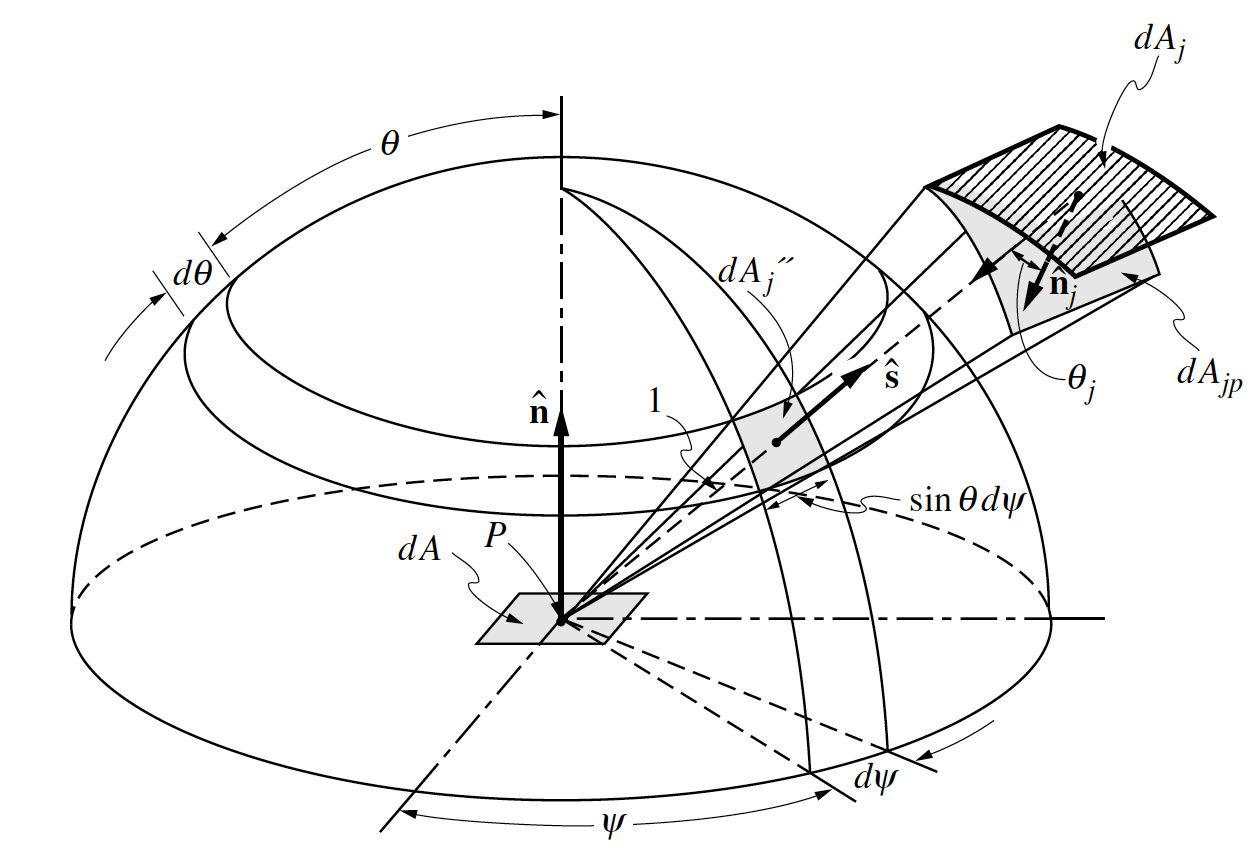
\includegraphics[width=\linewidth]{figures/ch3/solid_angl.png}
\caption{Angle definitions. $\theta$ is the polar angle, and $\psi$ is the azimuthal angle \cite{Modest2013RadiativeTransfer}. }
\label{fig:Unit_Sphere}
\end{figure}

Local thermodynamic equilibrium guarantees isotropic emission; therefore, integrand uniformity can be assumed and the relation simplified into eqs. \ref{eq:DirOfEmission_psi} and \ref{eq:DirOfEmission_theta}.
\begin{equation}
    \psi{} = 2\pi{}R_\psi{}
    \label{eq:DirOfEmission_psi}
\end{equation}
\begin{equation}
    \theta{}=\arccos{(1-2R_\theta{})}
    \label{eq:DirOfEmission_theta}
\end{equation}
Note the non-linear dependence of direction of the uniformly distributed random variable.

\subsubsection{Absorption}
The absorption processes within a cell can both be modeled in a similar fashion. The energy of a ray during its travel, or transmissivity $\tau{}$, in a non-scattering medium will deplete according to eq. \ref{eq:transmissivity}.
\begin{equation}
    \tau{}=\exp{\left(-\int^{l_\kappa{}}_0\kappa{}_\lambda{}~ds\right)}
    \label{eq:transmissivity}
\end{equation}
Therefore the random number relation for the absorption location of the ray can be defined as in eq. \ref{eq:discreteabsorption}.
\begin{equation}
    R_\kappa{}=\exp{\left(-\int_0^{l_\kappa}\kappa_\lambda{}\right)}
    \label{eq:discreteabsorption}
\end{equation}

The inverted equation can then be appropriately defined for a ray traversal through a series of $N$ discrete sub-volumes of uniform absorption coefficient, where complete ray absorption will occur at $i$th intersected cell as in eq. \ref{eq:discreteabsorption_cells}.
\begin{equation}
    R_\kappa{}=\exp{\left(-\sum{}_{i=1}^N\kappa_\lambda{}\Delta{}s_i\right)}
\end{equation}
\begin{equation}
    \sum{}_{i=1}^N\kappa_\lambda{}\Delta{s_i}=\ln{\frac{1}{R_\kappa{}}}
    \label{eq:discreteabsorption_cells}
\end{equation}

Where $\Delta{s_k}$ is the distance travelled through cell $k$. Because of the dependence of $\kappa{}$ on the ray's wavenumber and cell conditions, the exact cell where absorption will occur can only be modeled after the ray has been traced through the mesh, and the summation has been incrementally evaluated.

The absorption process can also be modeled using the energy 
partitioning approach, where eq. \ref{eq:transmissivity} is used directly in discrete form to define the gradual depletion of ray intensity. 
Then, each cell that a ray intersects will receive an energy defined be the difference of ray energy at the entrance and exit of the cell.
This approach is known to be more efficient in an optically thin medium where the rays will propagate far in the domain before complete absorption \cite{Modest2013RadiativeTransfer,Liu2020TheFlames}.

\subsubsection{Wavelength}
The random number relation for the wavelength can be described by eq. \ref{eq:RN_relation_wavelength}
\begin{equation}
    R_\lambda{}=\frac{\pi{}}{\kappa{}_p\sigma{}T^4}\int_0^\lambda{}\kappa{}_\lambda{}I_{b\lambda{}}~d\lambda{}
    \label{eq:RN_relation_wavelength}
\end{equation}

While the preceding relations for point of emission and direction of emission can be assumed uniform within a computational cell and across a unit sphere, the same assumption cannot be applied for the ray's wavelength. For most mixtures in combustion modeling, the emission spectrum will vary significantly with wavelength (see section \ref{Sec:Nongray}). 
Therefore, the inversion process of eq. \ref{eq:RN_relation_wavelength} is more complex.
A line-by-line accurate model of radiation requires a solution to the numerator through a high-fidelity spectroscopic database such as HITEMP \cite{Rothman2010HITEMPDatabase}.
One approach includes first evaluating the emission spectrum (integrand of the numerator), and tabulating the numerator incrementally from $\lambda{}=\lambda{}_{min}$ to $\lambda{}_{max}$.
Then, the wavelength corresponding to a random number can be determined through interpolation.

\subsection{Raytracing}
The MCRT method relies on a raytracing procedure to determine ray-cell energy deposition. This procedure requires calculations between every ray (tens of millions) with every cell that it intersects (several thousands). 
It is for this reason that raytracing is responsible for the bulk of the runtime consumed by the MCRT method.

Equation \ref{eq:transmissivity} requires knowledge of the order of cell intersection, as well as the distance travelled through each cell, $\Delta{}s$. While many structured meshes can evaluate tracing procedures using a fast pre-computing approach \cite{Amanatides1987ATracing}, when applied to mesh with cells of arbitrary number of sides, an additional layer of complexity is involved.
Only with both the distance travelled through a cell and the absorption coefficient can the fraction of ray energy that is deposited be calculated.
And only with a correct ordering of cell intersections can the non-linear exponential decay function of ray transmissivity be correctly integrated across the ray's path.
Therefore, the traditional approach to raytracing is to incrementally trace the ray through the mesh, one cell at a time, in order of intersection, as shown in algorithm  \ref{alg:traditional_raytracing}.

\begin{algorithm}[hbt!]
\caption{Pseudocode for the traditional ray tracing process through a mesh. No ray-boundary interactions, ray scattering, or parallel processing is accounted for.}\label{alg:traditional_raytracing}
\For{$emitting\_cell \in{} mesh$}{
    \For{$ray \in{} emitting\_cell.rays$}{
        \Call{ray.initialize}{~} \Comment*[r]{point of emission, direction, wavelength}
        $cell \gets emitting\_cell$\;
        \While{$ray.energy > energy\_minimum$}{\label{alg:line:depletion}
              $\Delta{s} \gets \Call{ray.get\_intsec\_length}{cell}$\;
              $\kappa{}_\lambda{} \gets$ \Call{cell.get\_absorption\_coeff}{$ray.wavelength$}\;
              $optical\_distance \gets \Delta{s}\times{\kappa{}_\lambda{}}$\;
              \State old\_energy $\gets$ ray.energy\;
              $ray.energy = ray.energy * \exp{(-optical\_distance)}$\;
              $cell.energy = cell.energy + (old\_energy - ray.energy)$\;
              $cell =$ \Call{ray.get\_next\_cell}{~}\;
        }
    }
}
\end{algorithm}

\subsubsection{Trigonometric Calculations}
Determining the distance travelled within a cell, $\Delta{s}$, requires trigonometric operations between the ray and each of the faces.
The calculation proceeds as follows. At its initial state, the ray is located within it's origin cell. Each face within this celll must be iterated through, and the distance the ray must travel to intersect the representative plane of each face can be calculated. 
Only the face which is the closest will be the exit face. 
The face can be modeled as an infinite plane with an outward-facing normal vector, $\Vec{\textbf{n}}$, and centerpoint, $\textbf{c}$.
And the ray has direction, $\Vec{\textbf{d}}$, and origin, $\textbf{p}$. 


The ray traversal can be described by eq. \ref{eq:ray_face_intersection}.
\begin{equation}
    \textbf{r} = \Vec{\textbf{d}}t + \textbf{p}
    \label{eq:ray_face_intersection}
\end{equation}
Where the location, $\textbf{r}$ is described by the distance traversed, $t$.
Meanwhile, the equation for a plane can be represented using eq. \ref{eq:eq_for_plane}.
\begin{equation}
    \Vec{\textbf{n}} \cdot (\textbf{r} - \textbf{c}) = 0
    \label{eq:eq_for_plane}
\end{equation}
Substituting eq. \ref{eq:ray_face_intersection} into eq. \ref{eq:eq_for_plane} creates the expression for $t$.
\begin{equation}
    t=\frac{d-\Vec{\textbf{n}}\cdot\textbf{p}}{\Vec{\textbf{n}}\cdot\Vec{\textbf{d}}}
    \label{eq:eq_for_plane}
\end{equation}
Where $d=\Vec{\textbf{n}}\cdot\textbf{c}$ \cite{Kay1986RayScenes}. This equation is calculated for every face in the polyhedron, and the exit face is determined through the minimum $t$ value. The exit face of a cell can then be used to determine the entrance face of the following cell using conveniently defined data structures.
The procedure then repeats until the ray has depleted sufficiently (algorithm~\ref{alg:traditional_raytracing}, line~\ref{alg:line:depletion}), or until a boundary has been intersected.

\subsubsection{Boundary Interactions}
The boundary interactions are dependent on the boundary conditions defined within the model. Three models are commonly implemented in MCRT: black boundary, gray boundary, and periodic boundary.

A black surface is one that absorbs all incident radiation, and emits according to Planck's law \ref{eq:PlancksLaw}. 
This could define a boundary to an open environment of surrounding, cold gas, a combustor boundary, or the high temperature boundaries of a rocket engine. 
Under these conditions, a ray which intersects this boundary will be absorbed in its entirety, and an absorption profile can be determined by accumulating energy depositions along the exit faces along the boundary. The emission from a black surface is diffuse, and therefore defined by the random number relations for a diffuse emitter, eqs. \ref{eq:diffuse_emission_psi} and \ref{eq:diffuse_emission_theta}.
\begin{equation}
    \psi{}=2\pi{}\R{}_\psi
    \label{eq:diffuse_emission_psi}
\end{equation}
\begin{equation}
    \theta = \arcsin{\sqrt{R_\theta}}
    \label{eq:diffuse_emission_theta}
\end{equation}

A gray boundary has a more complex interaction with the environment. Gray surfaces can absorb, reflect or transmit incident radiative energy back into the medium. Gray surfaces also have only a fraction of the emission as that of a black body.
The transmissivity, $\tau{}$, quantifies the portion of incident radiation that passes through the surface, the absorptivity, $\alpha$ is defined as the fraction of incident radiation that is absorbed; the reflectivity, $\rho$ is the fraction that is reflected. These definitions can be re-stated for a non-ideal, rough surface by replacing the -ivity suffix with -ance. 
Finally, from the emission perspective, the emissivity, $\epsilon$, is the ratio of emissive power to that of a black body.  Kirchoff's law (see section \ref{sec:KirchoffsLaw}) indicates that $\epsilon{}=\alpha{}$ under the conditions of radiative equilibrium.
Most surfaces do not transmit radiation, therefore, many surfaces can be represented by the relation $\rho{}=1-\epsilon$. 

Reflecting boundaries redirect incident rays from an incoming direction to an exit direction. 
The exit direction can be evaluated using either a diffuse or specular model. 
A diffuse reflection occurs when an incident ray is deflected back in a random direction into the medium. This is accurate for surfaces with a high degree of variability of surface norms (rough), and the exit direction can be evaluated using additional random number relations, eqs. \ref{eq:diffuse_emission_psi} and \ref{eq:diffuse_emission_theta}.
A specular reflection is one that occurs from a smooth material. 
An example would be a mirror, or the smooth surface of water. Under these conditions, eq. \ref{eq:specular_reflection} is used to model the exit direction, $\Vec{\textbf{d}_{e}}$, given the incident direction, $\Vec{\textbf{d}_i}$, and surface norm, $\vec{\textbf{n}}$.
\begin{equation}
    \Vec{\textbf{d}_e}=2(\Vec{\textbf{n}}\cdot\Vec{\textbf{d}_i})\Vec{\textbf{n}} -\Vec{\textbf{d}_i}
    \label{eq:specular_reflection}
\end{equation}

\section{Accelerated approaches to MCRT}

\subsection{Monte-Carlo reformulations}
The traditional forward-tracing approach provides a strong starting point to the understanding of Monte-Carlo ray tracing approaches. Alternative methods, however, have been proposed that provide unique advantages under various circumstances.
Many methods rely on an inversion of the radiation problem, so rays can be traced back to their point of origin, a concept that relies on the reciprocity principle of radiation \cite{Case1957TransferPrinciple}.

\subsubsection{Backwards/Reverse Monte-Carlo}
Oftentimes it is desired to evaluate the incident radiation upon a point or small surface, as opposed to the distribution of radiation throughout the domain.
Applying the forward-MC approach would result in be an exhaustive calculation, as only a small portion of the rays would reach the point of interest. It would be more convenient to exclusively compute rays which are known in advance to arrive at that point. 
Backwards Monte-Carlo provides a more efficient route for this type of problem.
Instead of tracing rays from their points of emission, rays are instead traced from their point of absorption.
In this approach, instead of allocating a ray-energy based on the emitting computational cell, rays are instead backtracked from the "destination cell", back to their "emission cell", while accumulating energy along the way.
This approach is common in radiation modeling, and can be applied to frozen-field problems \cite{}, transient radiative transfer problems \cite{Lu2004ReverseMedia}, and semi-transparent media \cite{Li2005BackwardSlab}.

The principle of reciprocity approach formally derived by \citet{Case1957TransferPrinciple} was expanded to include the effects of volumetric emission and absorption by \citet{Walters1992RigorousMedia}.
Further background regarding the method can be found in papers by \citet{Modest2003BackwardTransfer} and \citet{Howell2010ThermalTransfer}.

The RTE, eq. \ref{eq:RTE_Solution}, can be inverted for an incident ray traveling into a point, $-\hat{s}$.
\begin{equation}
    \begin{aligned}
    I_\eta{}(\textbf{r}_i,-\hat{s}_i) = &\epsilon{}_\eta{}(r_w)I_{b\eta{}}(r_w)\exp{\left[-\int_0^l\kappa{}(r')~dl'\right]}\\
    &+\int_{0}^{l}{ \left\{ \kappa_\eta(r')I_{b\eta}(r')\exp{\left[-\int_0^{l'}\kappa_\eta(r'')~dl''\right]} \right\}}~dl'
    \label{eq:Inverted_RTE}
    \end{aligned}
\end{equation}
Equation \ref{eq:Inverted_RTE} provides a method to now evaluate the radiative emission throughout the domain in reverse manner.
Assuming piecewise homogeneity, eq. \ref{eq:Inverted_RTE} can be reformulated into eq. \ref{eq:discrete_Inverted_RTE} to be solved stochastic form using the Monte-Carlo method.
\begin{equation}
    \begin{aligned}
    I_\eta{}(\textbf{r}_i,-\hat{s}_i)& = \epsilon{}_\eta{}(r_w)I_{b\eta{}}(r_w)\exp{\left[-\sum_{m=1}^M\kappa{}_{\eta{},m}(l_{m_{out}}-l_{m_{in}})~dl'\right]}\\
    &+\sum_{m=1}^M\left( I_{b\eta}(T_m)\left\{ \exp{\left[-\sum_{p=m_{out}}^M\kappa{}_{\eta{},p}(l_{p}-l_{p-1})\right]}- \exp{\left[-\sum_{p=1}^{m_in}\kappa{}_{\eta{},p}(l_{p}-l_{p-1})\right]} \right\} \right)
    \label{eq:discrete_Inverted_RTE}
    \end{aligned}
\end{equation}

Which leaves an equation which provides a physical description of the backtracking of a ray.
As the ray travels in the reverse direction, it will pass through a series of computational cells. 
As the ray is being traced, each computational cell intersected will contribute a portion of the net energy deposited to the cell of tracing origin. The energetic contribution of each of the passing cells is accounted for, alongside a transmissivity term to determine their contribution's decay before arriving at the destination cell (tracing origin).
In the end, there will be a ray whose accumulated intensity will be that which is deposited into the cell of tracing origin.
Provided a statistically significant number of ray samples, the net radiative absorption into the cell of tracing origin can be evaluated from the average.

INSERT AVERAGE EQUATION


\subsubsection{Reciprocal Monte-Carlo}
Several alterative methods were proposed by \cite{Tesse2002RadiativeApproach} and 

\subsubsection{Shift method}

\subsubsection{Null-collision Monte-Carlo}




\subsection{Adaptive mesh approaches}
The all-to-all nature of MCRT results in poor scaling with increasing mesh size. 
This is especially true when running large-scale simulations on distributed memory computers.
Ray-cell interactions may occur between a ray emitted on one side of the medium, and a cell located on the other side.
The resulting communication overhead required by the Message Passing Interface (MPI)\footnote{MPI is the parallel execution standard for distributed memory computers. It defines the syntax in C/C++/Fortran code used to communicate with other nodes in the high performance computer (HPC).}, can dramatically slow the computation. Additionally, the sequential nature of raytracing limits these MPI communications to an iterative sequence of communications between adjacent MPI ranks\footnote{An MPI rank, in this case, is an instance of a parallel execution process within MPI.}.
This results in a series of "MPI iterations" where rays are forced to wait at the boundary of one MPI rank before being communicated to the adjacent rank as a group. This wait time significantly reduces the performance of a Single Instruction Multiple Data (SIMD) parallel execution process, limiting the scalability of the model.

\subsubsection{Mesh Coarsening}
Mesh coarsening is one approach to alleviate this problem. The approach is to localize all mesh information within a node to prevent any MPI communications.
To store the full mesh on one node would violate the purpose of a distributed-memory simulation, so a mesh coarsening approach is imposed, where the mesh is less-refined at increasing distances from the point of emission.
The coarsened mesh reduces the memory load required to load the mesh. Several layers can be added of increasing the degree of coarsening further from node of interest. The concept capitalizes on the local nature of thermal radiation: 
while radiation can travel long distances, in many circumstances the radiation will have its most significant contributions local to the point of emission.
The following explanation follows that of \citet{Silvestri2019ASimulation}.

The transmitted radiative intensity through a mesh follows an exponential decay function of intersection length and absorption coefficient, proportional to
\begin{equation}
     I_{transmit} \sim \exp{\left(-\kappa{}_\lambda{}\Delta{s}\right)},
    \label{eq:specular_reflection}
\end{equation}
It is immediately apparent that the majority of ray absorption occurs at lower optical distances. This therefore suggests that a coarsening of the mesh at larger optical distances (further from the point of emission) can reduce computational runtime while maintaining a similar degree of accuracy.
The ray will be emitted and traced within the fine mesh locally, and transferred to a coarsened mesh after a prescribed number of grid steps.
Resulting, in total, for a reduced number of ray-cell calculations, and also the potential to store the entirety of the mesh on a single node, in a coarsened manor. 

The idea has been implemented a limited number of times, but with much success. \citet{Silvestri2019ASimulation} presented speedups approximately equal to the number of coarsened layers within a structured mesh, along with an method to optimally select the number of cells a ray should travel before coarsening. 
\citet{Humphrey2015ATracing} applied a similar concept to a gray reverse Monte-Carlo model within a structured mesh. \citet{Kelm2021TheTransport} applied the OpenFOAM-embedded LaGrangian particle tracking library to radiation transport in their solver, \verb|containmentFoam|, which uses a global mesh to prevent MPI communications.

Several possible issues remain within the method, however. For one, the requirement of a user specified number of grid steps inserts a certain degree of potential error into the calculation. 
The model is restricted in accuracy and applicability to only those who understand its limitations. A sufficiently general model could be applied under any circumstance, without user choice.
Additionally, the model has the potential to introduce TRI-related effects into the simulations. 
Even if appropriate averaging is conducted (averaging the complete emissive power term from each cell, weighted by cell volume) the usage of a spatially-averaging model is questionable for TRI-related studies, particularly within the context of absorption-TRI.
Finally, the implementation of a non-gray modeling with such models appears to be inefficient.

\subsubsection{Traversal Algorithms}


\textbf{Mesh Coarsening and Optimized Traversal}
and \citet{Kelm2021TheTransport}
\cite{Nery2011MassivelyTracing,Zeeb2001AnGeometries,Humphrey2015ATracing,Mazumder2006MethodsTransport,Saftly2013UsingNote,Kuczynskia2014RadiationBoundaries}


\subsection{Ray Tracing in computer graphics}
Many improvements to ray tracing have been introduced in recent years capitalizating on advancements in computational hardware and algorithms.
These improvements have largely been focused in the field of computer graphics, owing in large part to the dramatic increase in the need for fast and detailed visualization software \cite{Gupta2020CUDAComputing}. 
The vast knowledge obtained through extensive work to accelerate ray-tracing in computer graphics would be of significant value to many heat transfer researchers, but has historically been ignored \cite{Howell2021TheTransfer}. 
In particular, the increased involvement of the Graphics Processing Unit (GPU) has resulted in dramatic boosts in computational efficiency, but has been used relatively few times in radiation modeling.
Additionally, the bounding volume hierarchy (BVH) provides a optimal data structure to accelerate the geometric search procedure of the ray-tracing process.

\subsubsection{Graphics Processing Units (GPUs)}
GPUs offer high throughput for highly parallelizable, compute-bound problems.
GPUs differ from Central Processing Units (CPUs) because of the increased attention to hiding latency through raw data parallelism as opposed to minimizing cache access time. 
This Single Instruction Multiple Data (SIMD) approach is optimized because the GPU structure has more area dedicated to the data processing as opposed to the cache and control unit on the CPU \cite{Gupta2020CUDAComputing}.
At its origin, the GPU was used for the acceleration of graphical visualization of games and animation rendering. Today, GPUs are applied in vast number of fields for more general purposes (GPGPUs).

Computational scientists in particular have begun to take advantage of GPUs in their fields of study. In the hybrid computing model, a central processing unit (CPU) offloads compute-intensive and time consuming parts of the code to the GPUs.
By applying this model, users can selectively offload the necessary parts of the code to the GPU, while maintaining others on the CPU.

While many fields have seem considerable improvements with GPUs, thermal radiation modeling has seen them applied relatively few times. This comes as a surprise seeing that MCRT in particular carries many similarities to the ray-tracing in computer graphics.
\citet{Heymann2012GPU-basedAGN} applied GPUs to their thermal radiation simulations for radiation in active galactic nuclei.
\citet{Humphrey2012RadiationSystem} applied GPUs to the field of combustion, for their massively scalable code Uintah, where they have coupled their CPU-solved CFD with GPU-solved gray-model radiation \cite{Humphrey2015ATracingb,Humphrey2016RadiativeRefinement,Holmen2017ImprovingTasks,Peterson2018DemonstratingComputations}. 
\citet{Silvestri2019ASimulation}, finally, applied GPUs to combustion simulations with non-gray modeling, and were able to show 1000x speedups using the GPU with reverse monte-carlo and mesh-coarsening compared to CPU-run forward MC.

\subsubsection{Bounding Volume hierarchy}
At its simplest form, the bounding volume hierarchy (BVH) is a tree-based data structure which can be used to represent a series of objects in space \cite{Shirley2020RayWeek,Meister2021ATracing}. The usage in computer graphics is to detect intersections between a ray and a far-away object in logarithmic time (traversal through a tree), rather than linear time (test each object once at a time).

BVHs are constructed by first wrapping the objects in Axis Aligned Bounding Boxes (AABBs). In a cartesian coordinate system, the cornerpoints of this box can be determined by the maximum and minimum X, Y, and Z coordinates of the object.
This ensures that an intersection of the ray with the object cannot occur without an intersection of the ray with the bounding box. 
In practice, the ray-face intersection calculation needs to be fast, and the calculation between an axis-aligned face with a ray is the fastest \cite{Kay1986RayScenes}.

The object-level AABBs represent the leaf nodes of the binary tree. These boxes are then wrapped in further bounding-boxes, and the procedure repeats until there is one bounding box which wraps around the whole domain, which represents the root node of the BVH. 
For a binary tree, each node must have only two child nodes. The ray-tracing procedure can then proceed iteratively down the tree (rejecting nodes and their children which the ray does not intersect) until a final list of leaf nodes are left.

Graphics processing sees massive speedup with the use of the BVH data structure, especially with recent approaches using GPUs \cite{Nery2013ParallelGPGPUs,Meister2021ATracing,Karras2012MaximizingTrees}.
However BVHs see almost no usage in thermal radiation modeling \cite{Liu2020TheFlames}.
\citet{Kuczynskia2014RadiationBoundaries} for one, were able to accelerate computation of thermal radiation between faces with non-participating media. 
Also, \citet{Mazumder2006MethodsTransport} compared the BVH approach with a spatial-partitioning approach known as volume-by-volume advancement and found the BVH to be slower for surface-to-surface calculations. 
There apparently exist no applications of the BVH to participating media in thermal radiation modeling. Alternative approaches, such as the oct-tree approach, where a mesh is refined in regions of increased opacity, however, have been introduced and shown to provide significant speedups over linear ray tracing \cite{Saftly2013UsingNote}.

\section{Implementation for this study} \label{section:ModelForThisStudy}
In this research we capitalize on the proven speedup of GPUs to accelerate thermal radiation modeling, and attempt to additionally use the BVH data structure to provide speedup as well.
The flow chart in fig. \ref{fig:joint_flow_chart} describes the procedure followed by the current implementation of the radiation code.

\begin{figure}
  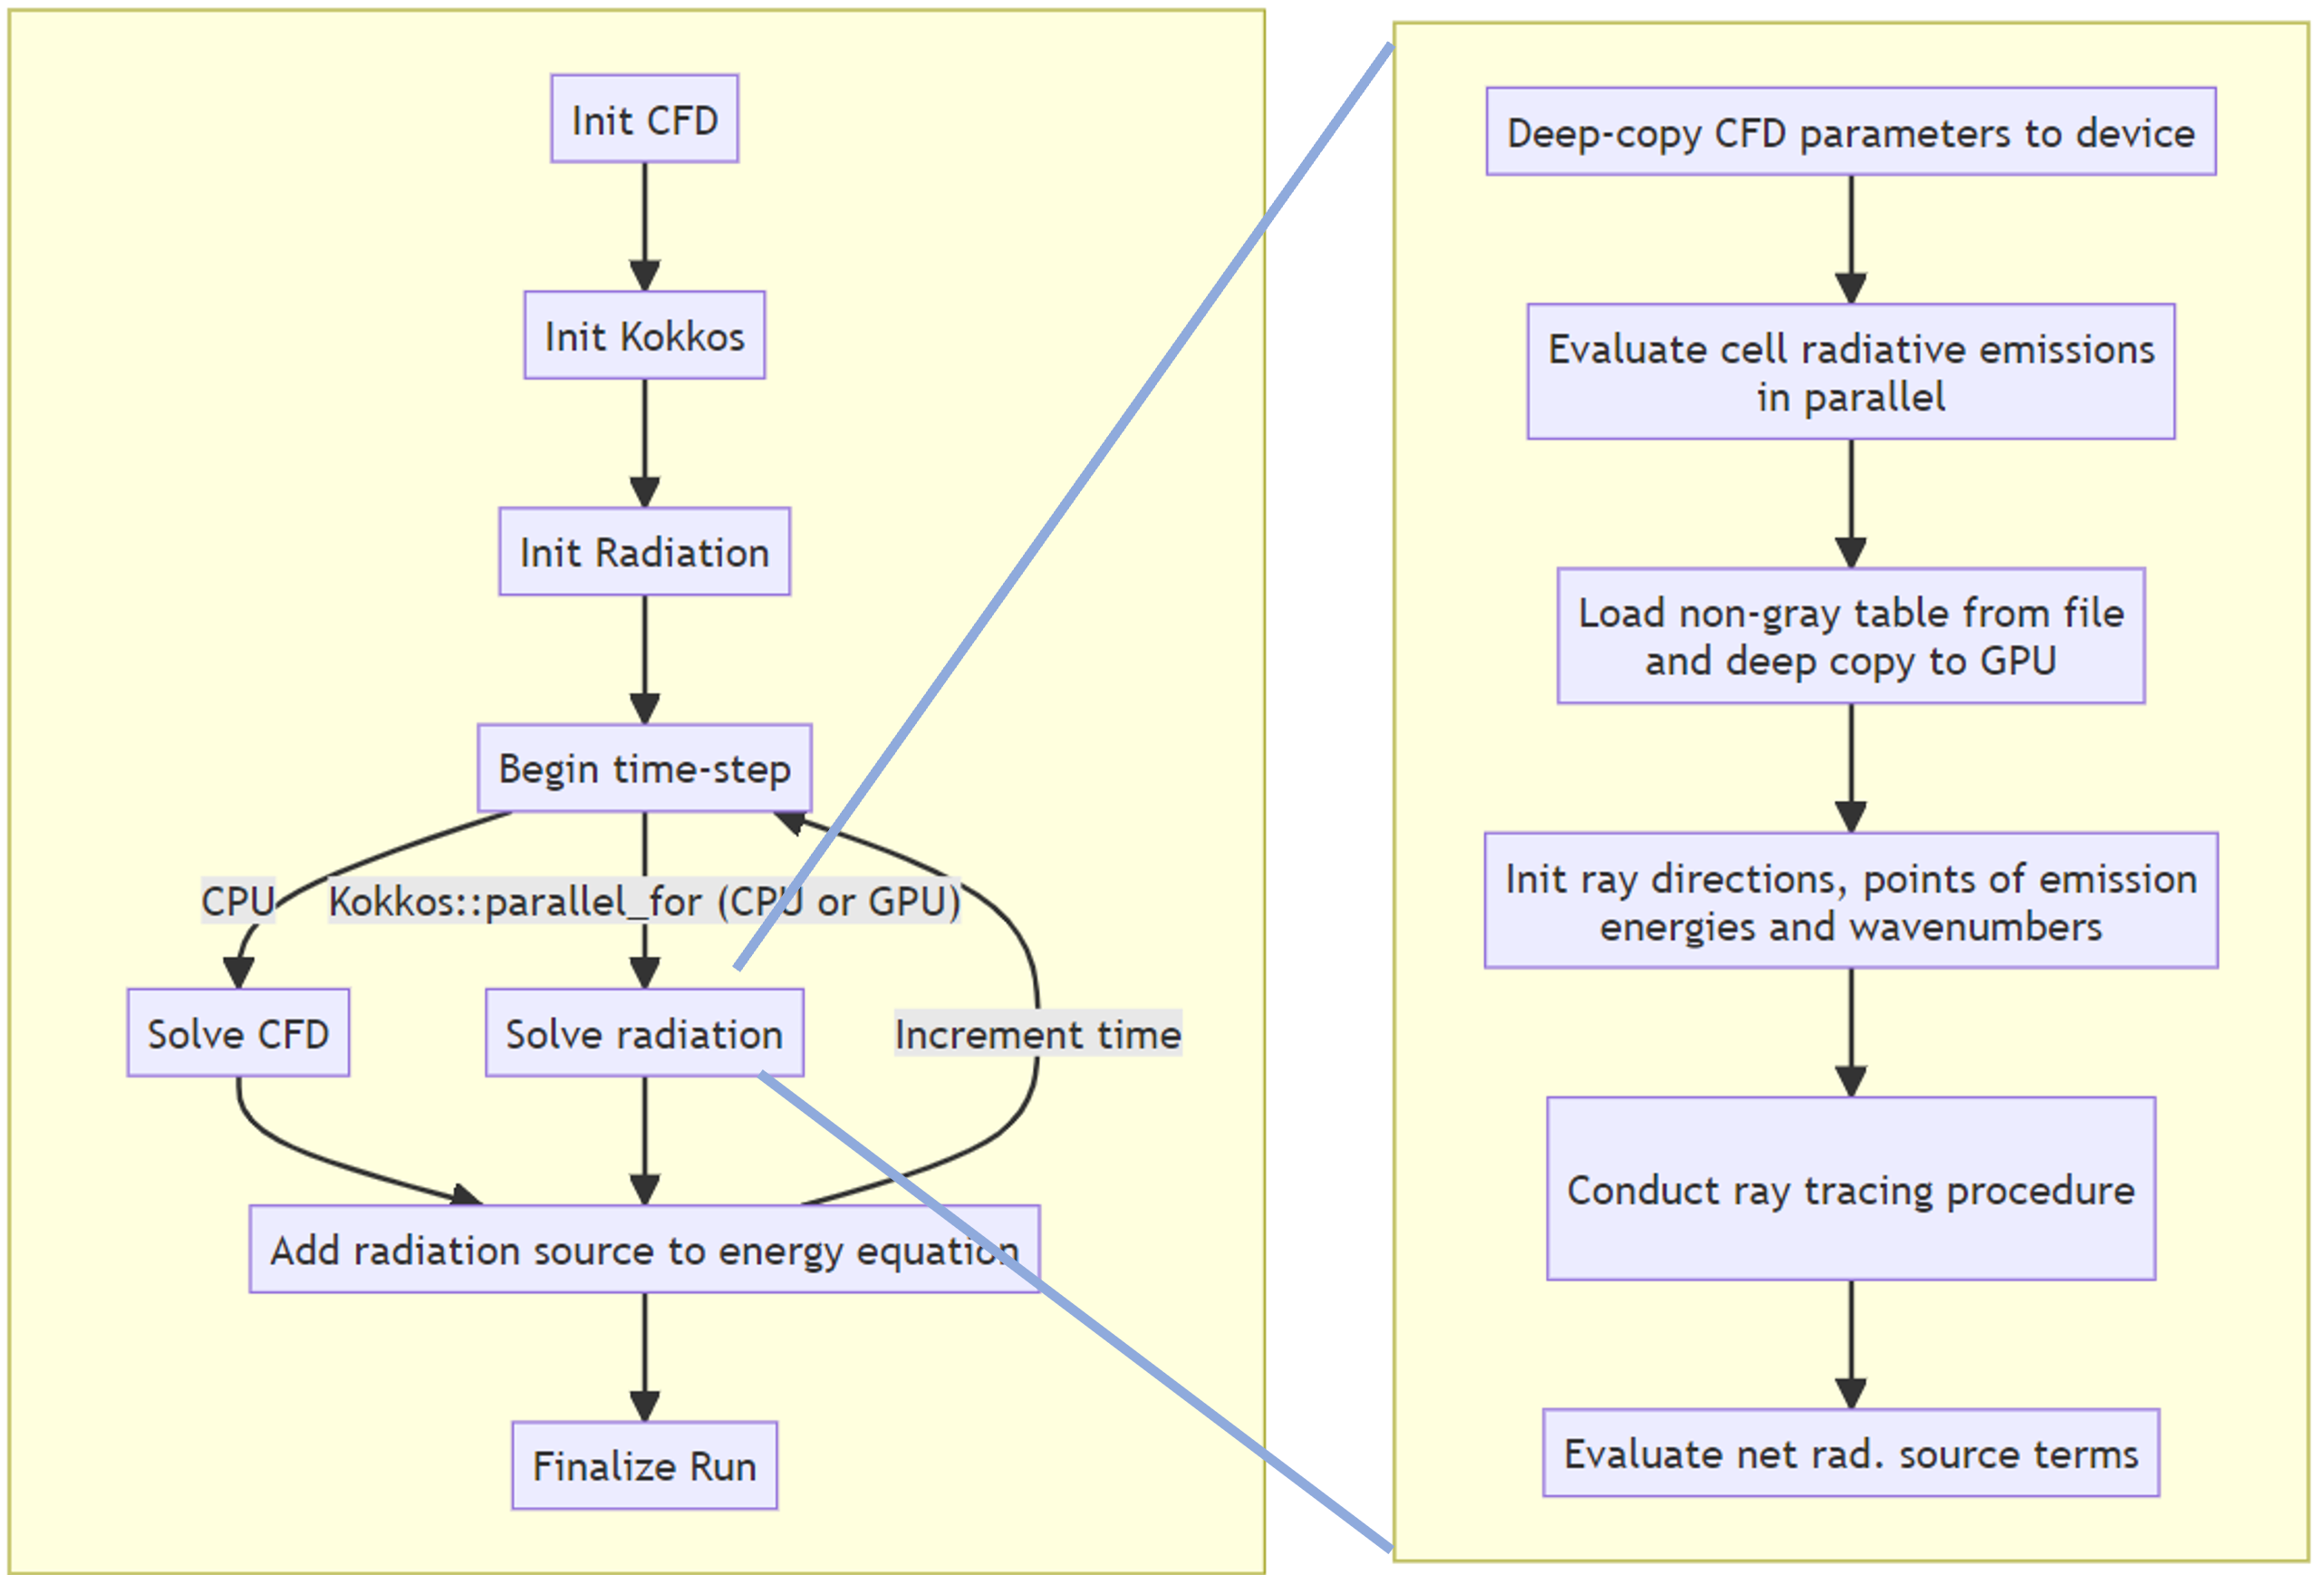
\includegraphics[width=\linewidth]{figures/ch3/joint_flow_chart.png}
  \caption{Diagram of MCRT implementation. The solver in its current implementation can solve radiation on the GPU and CFD on the CPU. Future work will include maintaining a fully asynchronous calculation using both CPU/GPU at the same time.}
  \label{fig:joint_flow_chart}
\end{figure}

\subsection{Description of the code}
Following the implementations discussed by \citet{Silvestri2019ASimulation} and \citet{Humphrey2015ATracing}, we implement an MCRT model on GPUs. 
This code connects to the OpenFOAM open-sourced CFD platform \cite{Weller1998ATechniques}, can run on distributed memory systems for scalable computation, and optionally uses a BVH to accelerate the geometric search process of the ray-box and ray-node intersections.
Our code consists of more than 3,000 lines of C++ code, and relies on the Kokkos programming model for a performance-portable parallelization framework \cite{Trott2021KokkosEra}, and the ArborX geometric search library for optimal BVH tree management and traversal functions (which itself relies on Kokkos) \cite{Lebrun-Grandie2019ArborX:Library}.


\subsubsection{OpenFOAM}
With OpenFOAM\footnote{https://github.com/OpenFOAM/OpenFOAM-5.x}, this code can be applied to any CFD solver of interest enabling its use in applications from aeronautical combustor engineering to fire suppression and management. OpenFOAM provides an extensive list of supplemental libraries, allowing the user to model RANS, LES, or DNS simulations with multi-phase flow and detailed chemistry. 
Time-accurate simulations can be implemented with MCRT-GPU with or without Adaptive Mesh Refinement (AMR) on polyhedral, unstructured mesh.
Users can adapt their own OpenFOAM solvers to use MCRT-GPU, or use the default examples for reactingFoam and fireFoam. Instructions are available in the public repository (or private?).

\subsubsection{Kokkos}
Kokkos~\footnote{https://github.com/kokkos} is a performance-portable programming model from the Department of Energy \cite{Trott_Kokkos3_2022,TrottKokkosOGPaper2014}. 
Targeted for HPCs, Kokkos provides abstractions over the parallel execution process and memory management in your solver. By programming in Kokkos, the user can neglect many worries about the underlying parallel execution process and instead focus on their code.
Kokkos supports CUDA, HIP, SYCL, HPX, OpenMP and C++ threads as parallel backends, which the user can easily switch between at compile time.
Additionally, the Kokkos ecosystem streamlines the debugging and profiling process \cite{Trott_KokkosEcosystem2021}.

\subsubsection{ArborX}
Following the Bounding Volume Hierarchy (BVH) description from \citet{Karras2012MaximizingTrees}, ArborX~\footnote{https://github.com/arborx/ArborX} provides a parallel implementation for both spatial-search and nearest-neighbor calculations using a BVH \cite{Lebrun-Grandie2019ArborX:Library}.

The ArborX API enables usage of the BVH through a two-step process: construction and traversal. The user can define \textit{primitives}, or underlying objects with labeled bounding-boxes, and ArborX will efficiently construct a balanced BVH for usage with any parallel backend (using Kokkos). Then, the user can define \textit{predicates} which define the operation the traversal process will be conducting (i.e. spatial search criteria) while traversing the tree.
MCRT-GPU enables the user to optionally use the BVH through ArborX to optimize the ray-tracing procedure. The \textit{primitives} are the computational cells in the CFD process (convex polyhedrons), and the \textit{predicates} are the rays traveling through space.

ArborX uses Kokkos as a backend for on-node parallelism, and implements additional MPI functionality to extend the BVH query process across multi-node runs. Distributed memory executions proceed through an upper-tree and lower-tree approach.
Each node contains knowledge of an upper-tree, which defines defines a BVH for each of the nodes in domain-decomposed space. Then, the lower tree represents the BVH for the computational cells that exist from the CFD solver. 
MCRT-GPU applies ray-tracing procedure across the distributed memory system using this method, which provides enhancement over the traditional MPI iteration approach as discussed in section \ref{sec:DistMemAccel}.

\subsubsection{Non-gray model}
MCRT-GPU has been built to enable use with one of three nongray models: line-by-line, gray modeling with a user-defined absorption coefficient, or gray modeling with planck-mean absorption coefficients. Non-gray databases have been previously derived from HITEMP \cite{Rothman2010HITEMPDatabase} including contributions of CO$_2$, H$_2$O, and CO spectral lines.


\subsubsection{User functionality}
MCRT-GPU is meant to be an adaptable radiation model that can be quickly linked to the user's OpenFOAM solver for fast and accurate radiation modeling during their time-accurate CFD simulation.

While the BVH may enable faster computation, in absence of proper development there exist both a version with and without its use.
The version without applies the traditional Monte-Carlo algorithms with Kokkos acceleration. This enables fast GPU-acceleration, with line-by-line non-gray modeling, ray-reflections, and distributed-memory calculation.

Users can access the code through a public repository on github \footnote{https://github.com/nick-jt/MCRT-GPU}.
\addchapheadtotoc
\chapter{Applied Radiation Model}\label{chapter:Example}
The complexity of the radiation solver resulting from both its theoretical foundation as well as its computational implementation calls for an extensive series of validation and performance studies.

Three test geometries are presented in this chapter for verification and profiling using the two methods discussed in section \ref{section:ModelForThisStudy}. The configurations include the canonical one-dimensional plane-parallel medium, a three-dimensional backwards-facing step combustor, and a three-dimensional Pratt \& Whitney NEO aeronautical combustor. 
These three test cases provide an excellent basis to verify the solution methods and test their performances. 



\section{One dimensional plane-parallel medium}
The plane-parallel medium provides a useful, one dimensional case to test the MCRT code. The geometry is shown in figure \ref{fig:PlaneParallelGeometry}.

The geometry consists of two parallel plates surrounding a radiatively-participating medium. The system is one-dimensional (implemented into OpenFOAM using either ray-reflections along the off-axis boundaries, or through a long stretch in both the Y and Z directions). The simulation is steady, and the walls are black-bodies (perfect absorbers and emitters).
Using this configuration, the user can artificially select an absorption coefficient, $\kappa{}$, medium temperature, $T$, and wall temperatures $T_w$.

Additionally, the relative simplicity of the configuration allows for reduced-complexity numerical solution described in appendix (IN APPENDIX OR PUT HERE?). 
This "analytical" solution can be used for verification of the solver under variable absorption coefficient, temperatures, and scattering coefficient (not included in this model).

The one-dimensional nature of the system also results in the least-ideal scaling for multi-node simulations. \textit{Provides useful understanding of how the runtime and memory usage scale for each solver under worst-case situations.}

\subsection{Results}
Figure \ref{fig:PP_kappatest} presents a comparison of the MCRT solutions alongside the analytical solutions. The configuration is tested under a variety of absorption coefficients, temperatures, and Monte-Carlo ray counts. The various case conditions are presented in table \ref{table:PPcomp}.

\begin{figure}
  \begin{subfigure}{1\textwidth}
  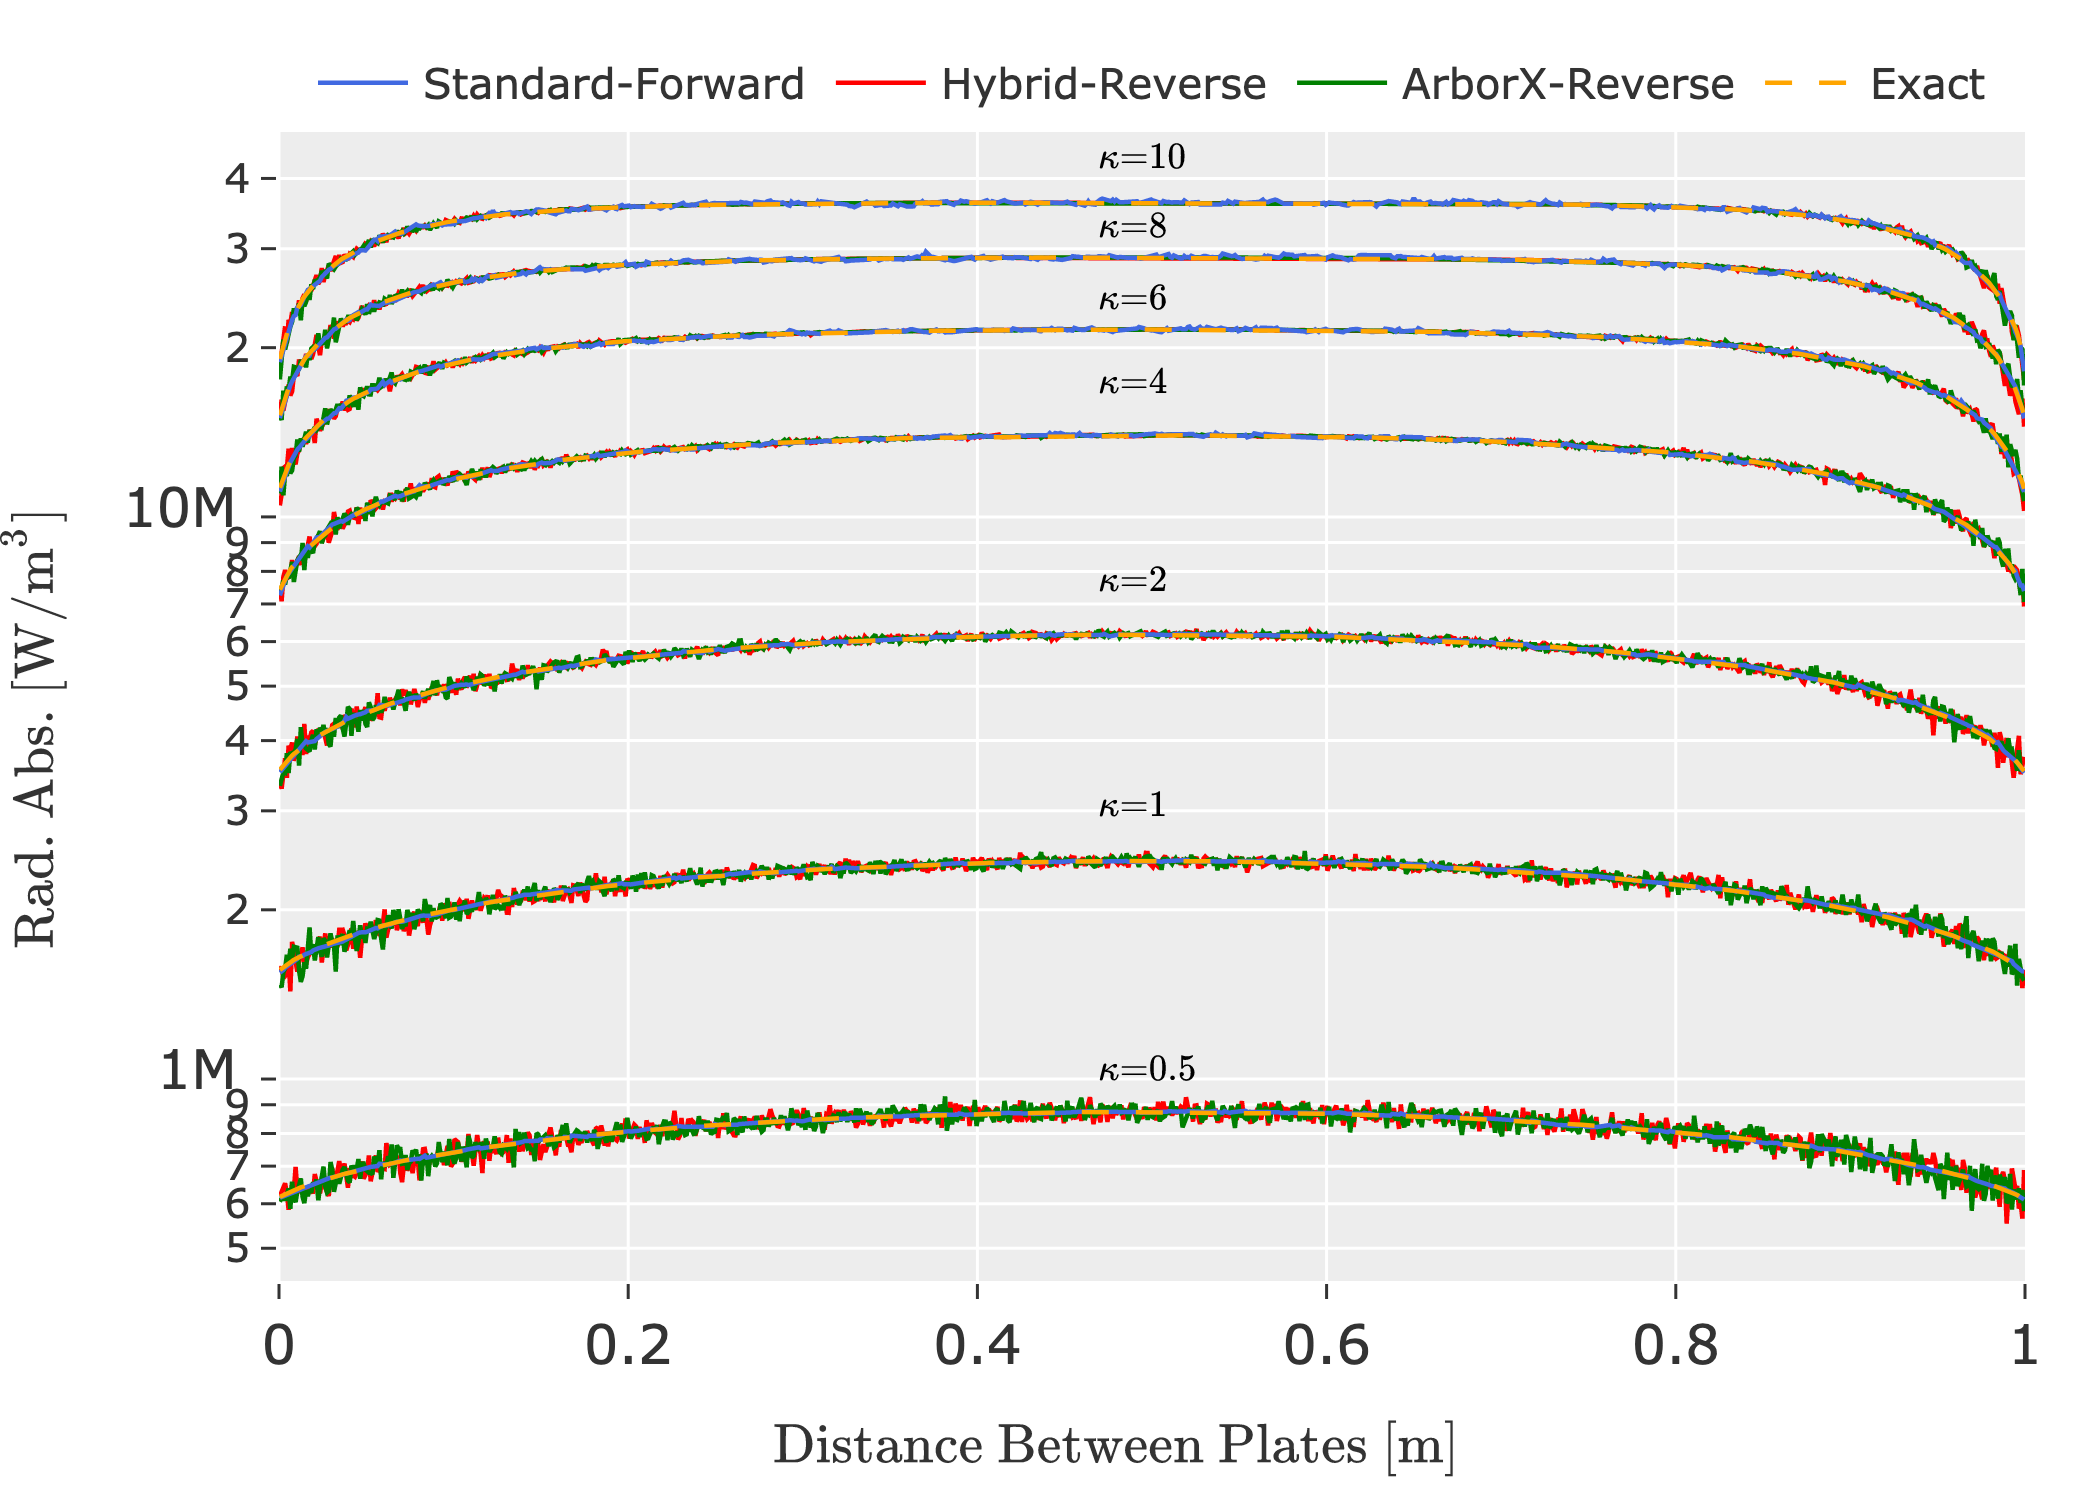
\includegraphics[width=\linewidth]{figures/ch4/PPcomparison1.png}
  \caption{Variable absorption coefficient with T=$2000$K, N$_r$=$1000$, N$_{cells}$=1000.}
  \label{fig:PPcomp_kappa}
  \end{subfigure}
  \begin{subfigure}{1\textwidth}
  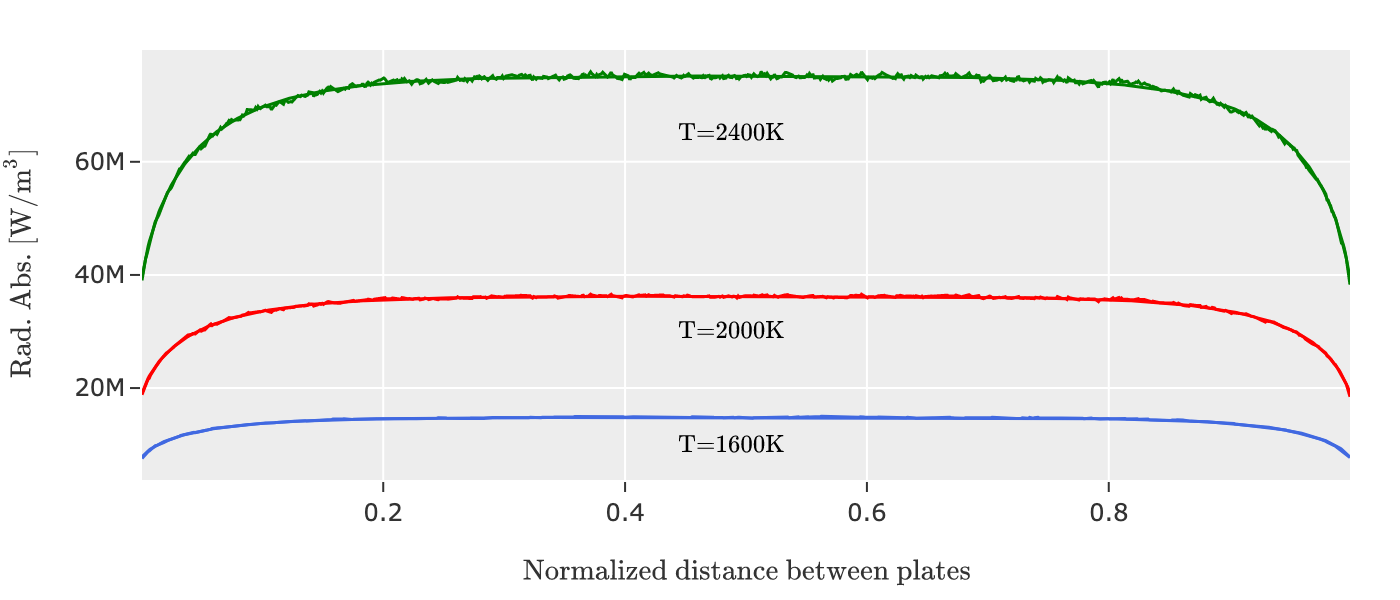
\includegraphics[width=\linewidth]{figures/ch4/PPcomparison2.png}
  \caption{Variable temperature with $\kappa{}$=$10$ m$^{-1}$, N$_r$=$1000$, N$_{cells}$=1000.}
  \label{fig:PPcomp_temp}
  \end{subfigure}
  \begin{subfigure}{1\textwidth}
  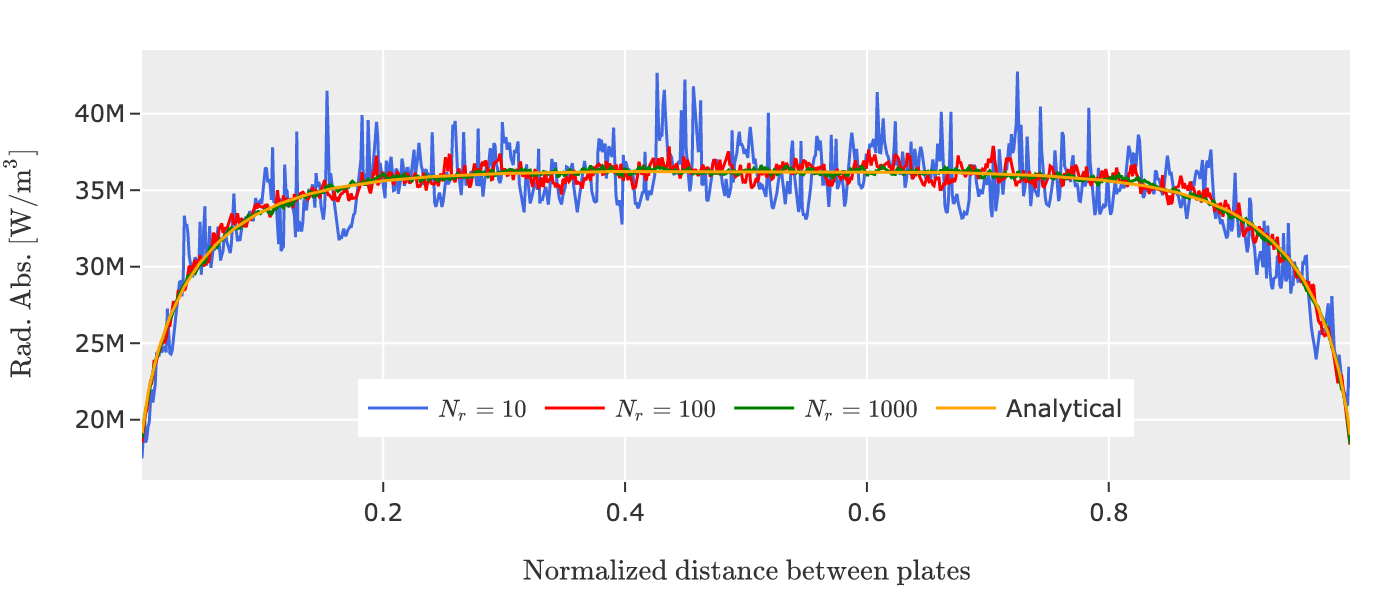
\includegraphics[width=\linewidth]{figures/ch4/PPcomparison3.png}
  \caption{Variable number of rays emitted per cell (N$_r$) with $\kappa{}$=$10$ m$^{-1}$, T=$2000$K, N$_{cells}$=1000.}
  \label{fig:PPcom_nrays}
  \end{subfigure}
  \label{fig:PPcomp}
\end{figure}

Results show excellent comparison between the MCRT and analytical implementations. 
The lower ray counts show a higher degree of variability resulting from the stochastic nature of the MCRT method. 
Increasing absorption coefficient leads in an increase of radiative emission and re-absorption, with re-absorption increasing at a higher rate resulting in a net increase of radiative source.

These expected results demonstrate the requirement for RTE modeling in optically thick media. Not only does radiative emission result in heat loss from computational cells, but also the re-absorption can be high enough to require modeling of the self-absorption process of radiation.

\subsection{Profiling}


\section{Backwards-Facing Step Combustor}
The backwards-facing step (BFS) combustor is a convenient geometry often used in the field of fluid dynamics for a simple, repeatable geometry to analyze turbulence, heat transfer and combustion.

\begin{figure}
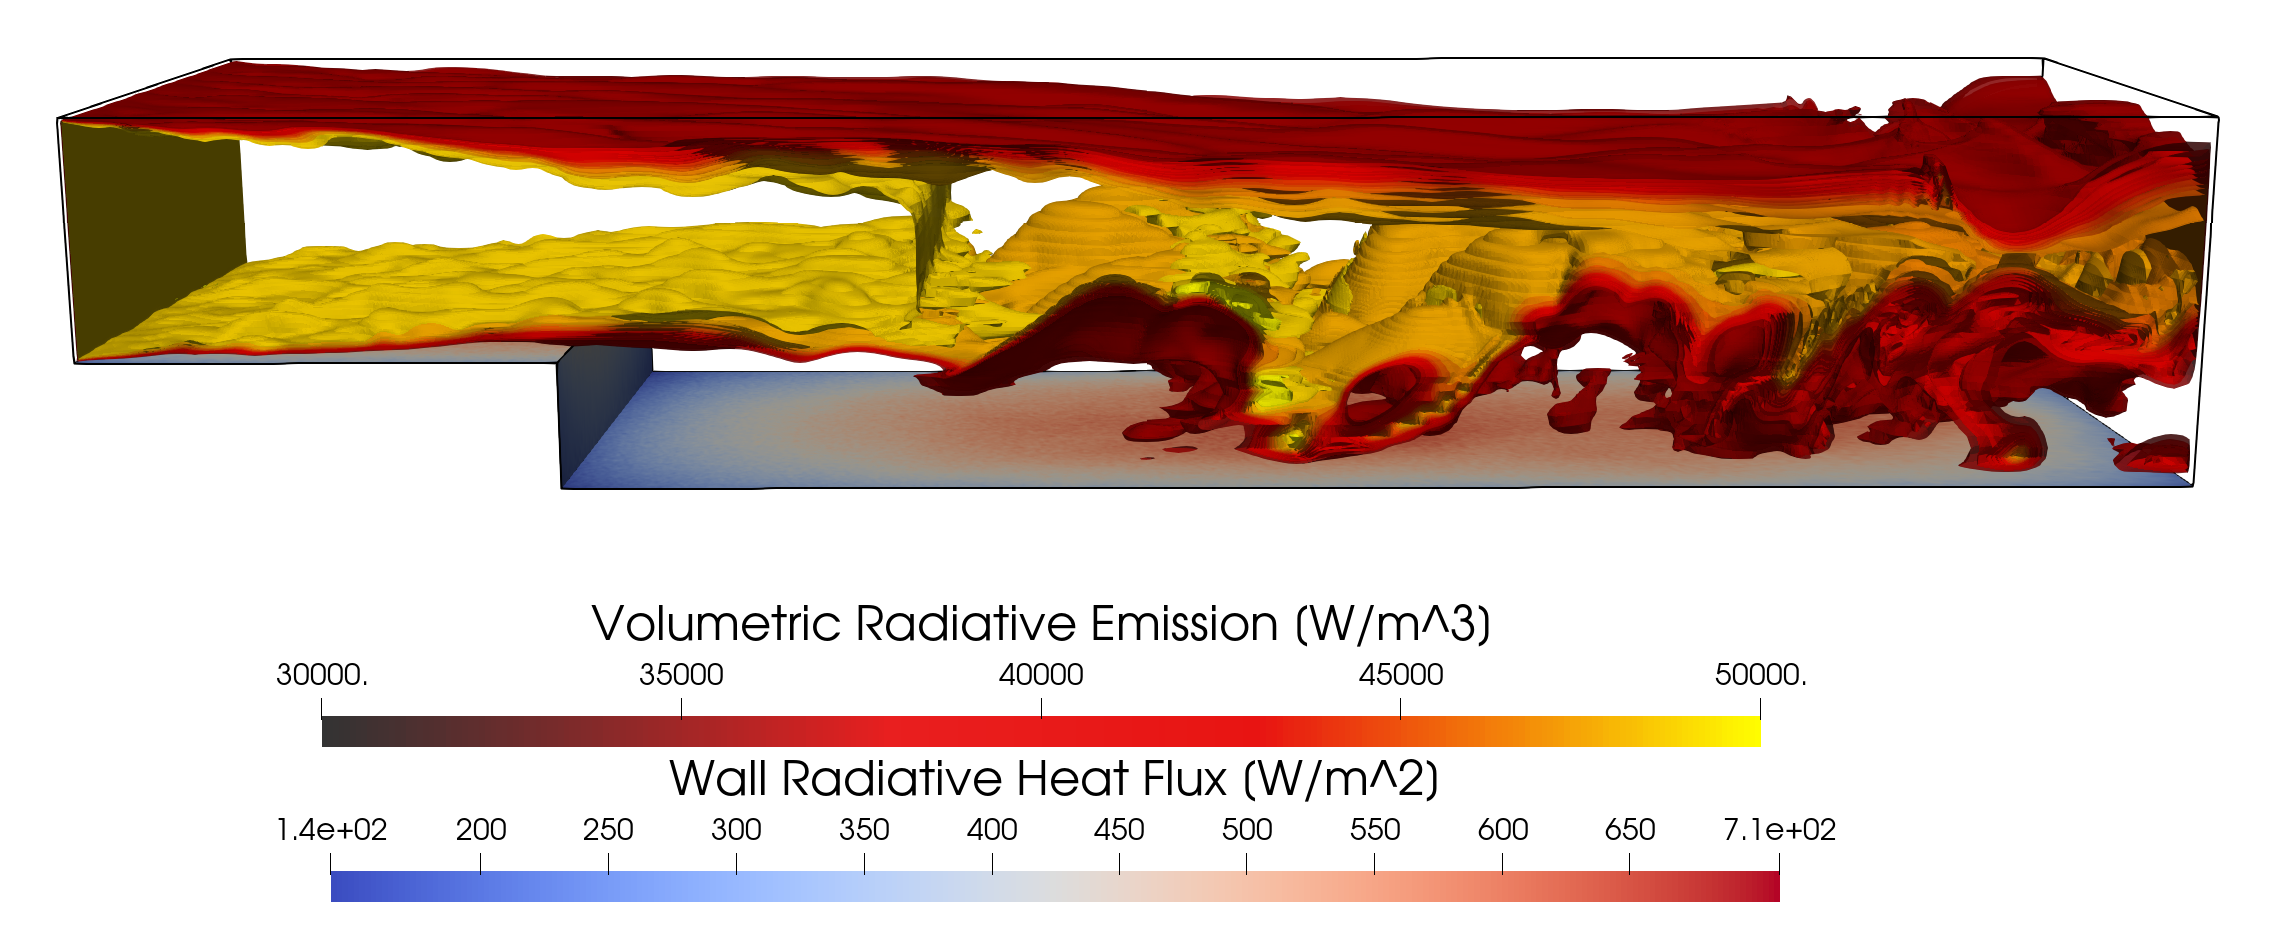
\includegraphics[width=\linewidth]{figures/ch4/BFS_volwallflux3.png}
\caption{Variable absorption coefficient with T=$2000$K, N$_r$=$1000$, N$_{cells}$=1000.}
\label{fig:BFS_geometry}
\end{figure}


\subsection{Background}
\subsection{Results}
\subsection{Model Performance}
\section{Pratt \& Whitney NEO Combustor or Pool Flame}

\addchapheadtotoc
\chapter{Conclusions and future work}~\label{chapter:conclusion}

\section{Summary of findings}
The influences of thermal radiation are known to be significant in combustion systems. A brief overview of the fundamentals of radiation, as well as categorized effects of radiation in combustion specifically, were discussed in chapter \ref{chapter:Importance}. 
Radiation has been shown to contribute significantly to changes in the turbulence, boundary interactions, and chemical characteristics in and around the flame.

TODO

The introduction of radiation in the modeling procedure will generally reduce temperatures of combustion processes. 
Additionally, it has been shown that the modeling of fire hazards, power generation devices, and many more applications require adequate modeling of radiation. 

The background of the Monte-Carlo method of modeling radiation was next discussed in chapter~\ref{chapter:Modeling}. The Monte-Carlo method is broadly known to be the most accurate, robust, but also most computationally expensive radiation model used.
With computational power increasing, however, it has been known to be the likely choice of the future. First an account of the fundamentals of MCRT, including the random number relations of point of emission, direction and wavenumber of the rays, was discussed.
A description of the tracing procedure through the mesh, and to the boundaries was also provided.
Several alternative mathematical techniques, as well as re-formulations of the Radiative Transfer Equation (RTE) were presented, along with their various advantages. Recent work has shown exciting progress, including the advent of the null-collision technique. Next, various influences of ray-tracing from the field of computer graphics were presented, including the Graphics Processing Unit (GPU) and Bounding Volume Hierarchy (BVH).
Previous literature was reviewed on applications of these methods, and it was found that relatively few researchers had applied GPUs to MCRT, but had observed tremendous runtime reductions, and almost no other researchers had applied the BVH to the calculation of a participating medium.
Finally, description of the radiation implementation for this research was presented, where both GPUs and BVHs were applied, as well as the highest fidelity non-gray model, line-by-line, and a robust tracing procedure through an unstructured polyhedral mesh.
The model was integrated with the \verb|OpenFOAM| CFD software package, which enabled its use with coupled, time-accurate combustion simulations through a source term contribution to the energy equation. Additionally, the Kokkos programming model and ArborX geometric search library were used for performance portability and BVH implementation, respectively.

The present model was applied to four geometries of varying complexity: a plane-parallel participating medium, a vitiated backward-facing step combustor, a turbulent time-accurate pool-fire, and a sooting Pratt \& Whitney combustor geometry.
First, the 1-D results showed excellent agreement with analytical solutions. Comparisons of the radiative absorption under a variety of absorption coefficients, medium temperatures, and ray counts showed expected results. Radiative absorption increased with absorption coefficient and temperature, and stochastic variability became more apparent with lower ray-counts.
Then, a 3-D backward-facing step combustor was simulated at a moderate temperature of approximately $800$K. Results were compared against those of an established Fortran-radiation model. Excellent agreement was found, further validating the new MCRT code. It was found that a runtime reduction of $60$\% was seen between the established Fortran implementation compared to the newer MCRT, and GPU parallel processing further reduced runtimes by approximately $25$\%. The speedups were a result of two advancements: improvements in parallel implementation through the introduction of the Kokkos back-end, and improved memory management through minimal duplication of mesh-data within the CPU.
Next, the 3-D pool-fire flame proved an excellent tool to demonstrate the use of the new MCRT model. First, a frozen-field analysis was conducted on an early timestep of the simulation. Results showed a strong redistribution of energy throughout the flame and to the surrounding walls. Trends between radiative absorption and emission with the Planck-mean absorption coefficient and flame temperature were outlined. A minimal degree of radiative absorption was seen in the surrounding medium. Additionally, the radiative re-absorption in the flame increased considerably when the line-by-line non-gray model was implemented. Detailed account of runtime consumption in the model was described through the use of a profiling tool. It was found that a significant portion of the runtime was consumed through the loading and transferal of the non-gray database. These results were magnified for the GPU, where a deep copy must be performed.
The same configuration was then run from initial conditions in a time-accurate simulation. Physical interpretability of these results were expected to be more accurate because correct influences of radiation can only be accounted for by simulating from initial conditions. Results showed a significant decrease in temperature of up to $600$K compared to the simulation without radiation. Profiling results displayed a consistent $25$\% of the runtime was consumed by radiation for each time-step, on average. Noting the results from the profiling of the frozen-field analysis, it was concluded that the consumption in runtime would decrease if the radiation database is maintained in memory between time-steps.
Finally, succesful validation of the present radiation model encouraged the modeling of a Pratt \& Whitney NEO combustor with line-by-line accurate non-gray modeling. A scatter diagram of various computational parameters in the medium revealed soot exerted a controlling influence on the radiation emission characteristics in the flame. At temperatures beyond a crossover point, soot volume fractions diminished rapidly, resulting in an equally rapid decrease in radiative emission, leading to a local maximum in radiative emission as a function of temperature. The boundaries of the combustor displayed a much higher degree of radiative heat flux adjacent to the fuel-rich region of the combustor. The influence of non-gray modeling was then presented. The line-by-line non-gray model as shown to increase radiative re-absorption significantly and decrease wall-incident radiative heat flux by up to $60$\%. The contributions of various chemical species to the wall-incident heat flux was evaluated, and it was found that soot contributed the most, followed by CO$_2$. 
Profiling of the radiation model on the combustor showed a reduction of runtime by approximately 75\%, and the non-gray calculation increased runtimes by 10\%.

\section{Recommendations for Future Work}
The present implementation of MCRT showed significant speedup compared to the established code. However, it is anticipated that further speedups can be obtained by implementing improved GPU-favorable memory and execution coherence \cite{Silvestri2019ASimulation}, and through the introduction of accelerated distributed memory approaches \cite{Humphrey2015ATracing}. A fully asynchronous computation of radiation and CFD on the GPU and CPU simultaneously would significantly reduce the apparent runtime of radiation. Furthermore, the potential for the Bounding Volume Hierarchy was limited in the present demonstration, however, the BVH may have potential to provide improvements for a distributed-memory simulation. Specifically, the tracing of a ray may proceed simultaneously within multiple GPUs at once through an all-at-once all to all communication of radiation. This implementation of the BVH will be explored in future studies.
Additionally, the potential for the described advanced Monte-Carlo reformulations have been shown to improve runtimes, and may carry significant advantages computationally. Implementations into the current model would likely lead to further performance improvements. Finally, the potential for the null-collision MC technique has only recently been revealed, and it may therefore have significant potential for the acceleration of MCRT. Combining this method with advanced mesh approaches, such as the BVH, could bring measurable speedups to the ray-tracing calculation.
These improvements would enable scientists and engineers to have more complete understanding of the influence of radiation within their combustion systems. 
%\chapter{Using Maintext Format}
\section{Section}

\chapter{Using Main Format}
\section{Section}


% Appendices
\appendix

%%%%%%%%%% DON'T DELETE THIS, REVERTS NUMBERING BACK %%%%%%%%%%%%%
\makeatletter
\renewcommand{\@makechapterhead}[1]{\vspace *{-10\p@ }{\parindent \z@ 
\raggedright \normalfont \ifnum \c@secnumdepth >\m@ne \Huge \bfseries 
\@chapapp \space \thechapter \vskip 10\p@ \fi #1\par \nobreak \vskip 30\p@ }}
\makeatother
%%%%%%%%%% DON'T DELETE THIS, REVERTS NUMBERING BACK %%%%%%%%%%%%%





\chapter{Analytical Solution for a plane-parallel medium}
\vspace*{-0.3in}

\section{Formulation}

\section{Numerical Approach}


\chapter{Appendix chapter 2}\label{appendix:machLearning_suppMaterials}





% Bibliography
\begingroup
%    \setlength\bibitemsep{10pt}
    \linespread{1}\selectfont

    \bibliographystyle{abbrvnat}
    
\bibliography{references}
\endgroup
%\addcontentsline{toc}{part}{References}

\end{document}
